\section{Decision explanation}
\label{sect:explain}
This section describes the explanation extraction process to identify the relevant frequency bins for the segmentation.

\subsection{Explanation extraction}

The proxy model is built on the NMF framework.
This allows to map the $\mathbf{H}=[\mathbf{h}_1,\cdots,\mathbf{h}_t,\cdots,\mathbf{h}_T]$ embedding to the frequency domain.
Furthermore, the segmentation prediction is obtained from this embedding with the $\Theta$ linear transformation.
The first step in the explanation process is to identify the $k\in [1,\cdots, K]$ NMF components that are the most relevant for classification.
We first apply a pooling operation to the embedding by averaging it over the time dimension: $z_k = \frac{1}{T}\sum_{t=1}^T \mathbf{h}_t$.
To identify the relevant components to detect the class $c$, we define a relevance vector $\mathbf{r}_c=[r_{1,c}, \cdots, r_{k,c}, \cdots r_{K,c}]$ in which each element is computed as:
\begin{equation}
    r_{k,c} = z_k \times \theta_{k,c},
    \label{eq:relevance_vector}
\end{equation}
where $\theta_{k}$ is the $k$-th weight of the linear layer associated to class $c$.

The most relevant components are selected by applying a threshold $\tau$ to \eqref{eq:relevance_vector}. 
A filtered relevance vector $\mathbf{R}_{c,\tau}$ is obtained, in which the $k$-th element is defined as:
\begin{equation}
    R_{k,c,\tau} = 
    \begin{cases}
        r_{r,k} & \text{if } r_{r,k} > \tau \\
        0       & \text{otherwise}. \\
    \end{cases}
\end{equation}

\subsection{Segment-level explanation}

The filtered relevance vector $\mathbf{R}_{c,\tau}$ belongs to the same space as the $\mathbf{H}$ embedding.
Hence, it can be projected to the frequency domain by the following NMF linear transformation:
\begin{equation}
    \mathbf{X}_{c,\tau} = \mathbf{W}\mathbf{R}_{c,\tau},
    \label{eq:rel_proj_freq}
\end{equation}
where $\mathbf{X}_{c,\tau}\in\mathbb{R}^{K}$ is the projection of the relevant components in the frequency domain given $c$ and $\tau$.
This representation highlights the relevant frequency bin to detect a given class.

After identifying the relevant components, it is necessary to measure the confidence in the model decision.
The confidence measure is obtained by only keeping the relevant components in the $\mathbf{H}$ embedding and forwarding this filtered embedding $\mathbf{H}_{c,\tau}$ through the $\Theta$ layer such that $\tilde{\mathbf{y}}_{c,\tau}=\Theta(\mathbf{H}_{c,\tau})$.
Thus, the frequency-domain explanation $\mathbf{X}_{c,\tau}$ can be compared to the model output for a given threshold $\tau$.

\begin{figure}[ht]
    \centering
    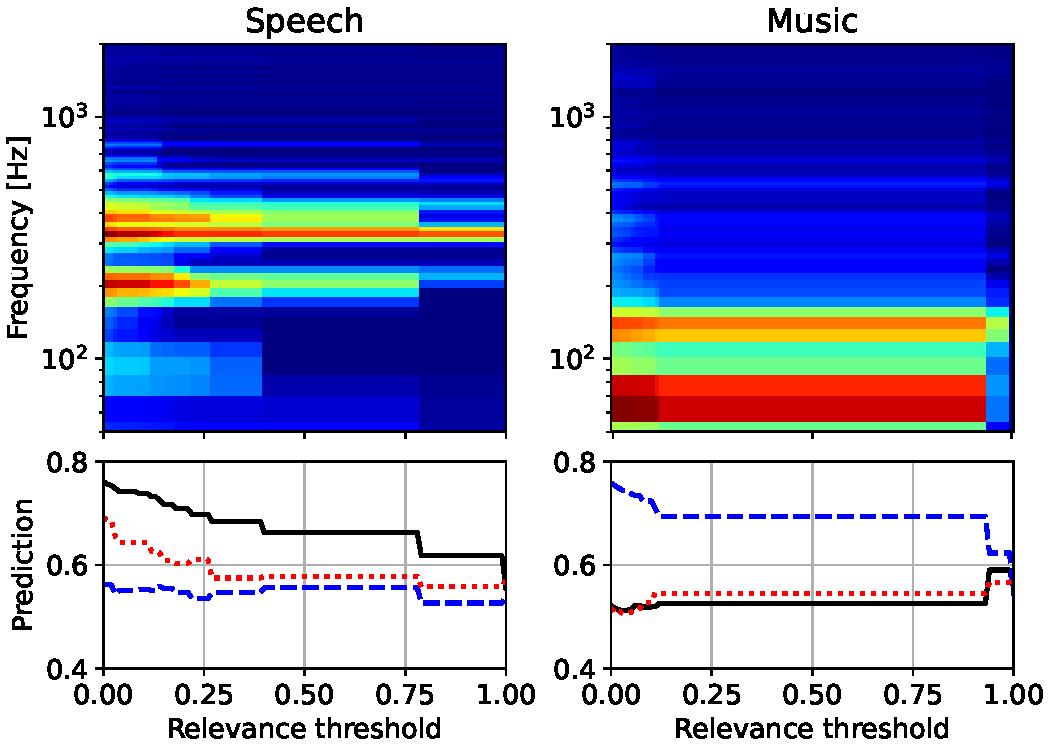
\includegraphics[width=\linewidth]{figs/icassp_rkc.pdf}
    \caption{(Top) relevant for speech and music segmentation according to the relevance threshold $\tau$. (Bottom) Model prediction for (\textbf{--}) speech, (\textbf{\textcolor{blue}{-~-}}) music, and (\textcolor{red}{$\boldsymbol{\cdots}$}) overlapped speech with each selected components.}
    \label{fig:seg_explain}
\end{figure}

Figure \ref{fig:seg_explain} shows the relevant components projected in the frequency domain with the equation \eqref{eq:rel_proj_freq} for two types of segments: speech and music.
The relevant components are presented as a function of the relevance threshold.
The model prediction obtained from the selected components is also presented.

The figure shows that the relevant components for speech are located between 100Hz and 1kHz. 
The model shows a high prediction until $\tau=0.75$. 
This allows to identify of the most relevant components for speech classification e.g., the component around $f=$200Hz.
The overlap prediction is also affected by these components.
This can be explained by the presence of common relevant frequency bins between SAD and OSD (Fig. \ref{fig:global_exp}).
However, the music prediction is similar for each $\tau$, demonstrating that the identified frequency bins are not used for MD.

In the case of MD, the relevant frequency bins are located between 50Hz and 200Hz.
The components located in the band [60,80]Hz are highly relevant for music detection.
When those are removed ($\tau$=0.9), the music prediction drops.
SAD and OSD prediction remain similar for each $\tau$ since the frequency bins are different between music and these classes.

The quality of the reconstruction limits the explanation extraction in the frequency domain.
In the case of the Wavlm-based proxy model, the reconstruction is of low quality in high frequencies. 
Thus, no explanation can be extracted in this part of the spectrum.
The following section proposes to extend the relevance component identification by global analysis.

\subsection{Global explanation}

The proposed explanation is obtained at the segment level, meaning that the relevant components are identified locally.
However, there is no guarantee that the components used to detect a class $c$ in a segment are the same across an entire dataset.
Thus, we propose a global explanation, which averages the relevance vectors $\mathbf{r}_{c}$ for a set of $N$ segments $\mathcal{D}_c=\{\mathbf{x}_{1,c}, \cdots, \mathbf{x}_{n,c}, \cdots \mathbf{x}_{N,c}\}$ containing the class of interest $c$:
\begin{equation}
    \bar{\mathbf{r}}_{c} = \frac{1}{N}\sum_{\mathbf{x}_{c}\in\mathcal{D}_c} \mathbf{r}_c.
    \label{eq:avg_rel}
\end{equation}

The $\bar{\mathbf{r}}_{c}$ vector highlights the global relevant components to detect the class $c$.

\begin{figure}[htb]
    \centering
    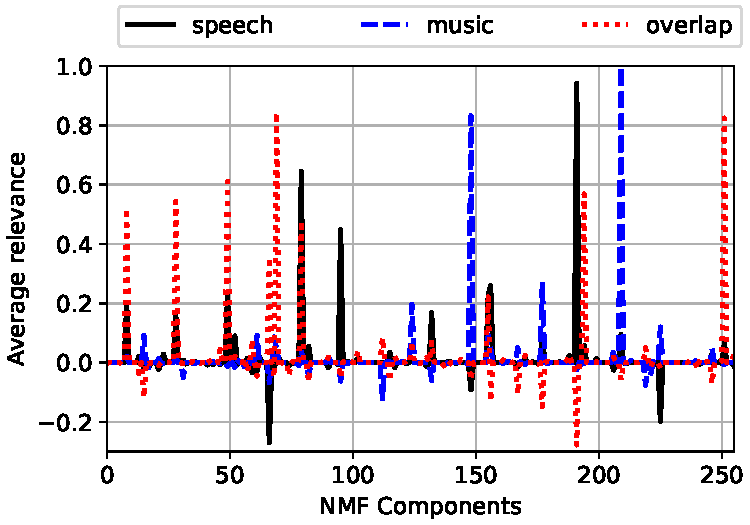
\includegraphics[width=0.8\linewidth]{figs/r_kc_acc.pdf}
    \caption{Global relevant components for speech (sp), music (mu), and overlapped speech (ov).}
    \label{fig:global_exp}
\end{figure}


To compute the average relevance of equation \eqref{eq:avg_rel}, 100 segments containing exclusively each class of interest are selected to build each subset $\mathcal{D}_c$.
To better control the OSD case, two-speaker artificial speech mixtures are generated by summing two speech segments.
The noise class is not represented since few segments contain exclusively noise.

Figure \ref{fig:global_exp} presents the average relevance $\bar{\mathbf{r}}$ for each NMF component,  computed for SAD, OSD, and MD.
It shows that some NMF components are typical for SAD and OSD.
For example, the component of index 50 is activated for both classes.
In contrast, some components discriminate between these two classes e.g., at index 70 where the speech component shows a negative relevance.
The figure also demonstrates that the NMF components related to music are different from speech and overlap ones.
This confirms the behavior observed at the segment level in figure \ref{fig:seg_explain}.
